\documentclass[12pt]{article}

\usepackage{sbc-template}
\usepackage{graphicx,url}
\usepackage[utf8]{inputenc}
\usepackage[brazil]{babel}
\usepackage{tikz} %Ferramenta mais complexa e poderosa para criar elementos gráficos
\usetikzlibrary{calc}
\usepackage{tkz-fct,tkz-euclide,tkz-base,tikz}
\tikzset{bolinha/.style={circle, draw, fill=none,
		inner sep=1pt, minimum width=1pt}}
\tikzset{bola/.append style={circle, draw, fill=none,
		inner sep=2pt, minimum width=1pt, fill=gray!50}}

\usepackage{colortbl}
\usepackage{booktabs}
\usepackage{hhline}
\usepackage{array}
\usepackage{color}

\tikzset{
	square/.style={%
		draw=none,
		circle,
		append after command={%
			\pgfextra \draw[black] (\tikzlastnode.north-|\tikzlastnode.west) rectangle 
			(\tikzlastnode.south-|\tikzlastnode.east);\endpgfextra}
	}
}

%Interface para algoritmos%
%%%%%%%%%%%%%%%%%%%%%%%%%%%%%%%%%%%%%%%
\usepackage{algorithm}
\usepackage{algpseudocode}
%%%%%%%%%%%%%%%%%%%%%%%%%%%%%%%%%%%%%%%%%%%%%%%%%%
\usepackage{hyperref}
\hypersetup{
	colorlinks=true,
	linkcolor=blue,
	filecolor=blue,      
	urlcolor=blue,
	citecolor=black,
	% pdftitle={Overleaf Example},
	% pdfpagemode=FullScreen,
}
     
%\sloppy

\title{Proposta de projeto: Monte Carlo e Cadeias de Markov}

\author{Amanda Ferreira de Azevedo\inst{1}, Wanderson Lomenha\inst{1}}


\address{
	Universidade Federal do Rio de Janeiro\\
	Instituto Alberto Luiz Coimbra de Pós-Graduação e Pesquisa em Engenharia\\
	Programa de Engenharia de Sistemas e Computação
	\email{\{afazevedo,wanderson\}@cos.ufrj.br}
}

\begin{document} 

\maketitle

%\begin{abstract}
%  This meta-paper describes the style to be used in articles and short papers
%  for SBC conferences. For papers in English, you should add just an abstract
%  while for the papers in Portuguese, we also ask for an abstract in
%  Portuguese (``resumo''). In both cases, abstracts should not have more than
%  10 lines and must be in the first page of the paper.
%\end{abstract}
%     
%\begin{resumo} 
%  Este meta-artigo descreve o estilo a ser usado na confecção de artigos e
%  resumos de artigos para publicação nos anais das conferências organizadas
%  pela SBC. É solicitada a escrita de resumo e abstract apenas para os artigos
%  escritos em português. Artigos em inglês deverão apresentar apenas abstract.
%  Nos dois casos, o autor deve tomar cuidado para que o resumo (e o abstract)
%  não ultrapassem 10 linhas cada, sendo que ambos devem estar na primeira
%  página do artigo.
%\end{resumo}

\section{Definição do problema}


Seja $G = (V, E)$ um grafo simples, conexo e não orientado, onde V é o conjunto de vértices e E é o conjunto de arestas. Associe um custo não-negativo $c_e$ à cada aresta $e = \{i,j\} \in E$. Denota-se por $d_{ij}$ ao comprimento do menor caminho simples ligando os vértices $i,j \in V$, ou seja, à \textit{distância} entre eles no grafo $G$. Por fim, o \textit{diâmetro} de $G$, $d$, é dado pela maior distância existente entre qualquer par de vértices de $G$, em termos de número de arestas. Além disso, seja \textit{B} um número positivo que impõe um limite superior para o quanto se pode gastar na escolha das arestas de uma árvore geradora $T = (V_T, E_T)$. Denomina-se por \textit{Budget Minimum Diameter Spanning Tree Problem} (BDSTP) o problema de encontrar uma árvore geradora $T$ tal que a soma total de suas arestas não ultrapasse $B$ e seu diâmetro seja o menor possível. O problema foi proposto por \cite{Plesnik1981}, sob uma denominação imprecisa onde foi identificado como NP-Difícil. Uma ilustração de uma árvore geradora ótima para o problema é dada na Figura \ref{fig2}. 

\begin{figure}[ht]
	\begin{center}
		\begin{tikzpicture}
			[scale=1.5,auto=left]   
			\tikzstyle{every node}=[circle, draw, fill=white, inner sep=0pt, minimum width=17pt]
			\node[fill=gray!50]  (a) at (0.5,2) {a};
			\node[fill=gray!50]  (b) at (1,2.5) {b};
			\node[fill=gray!50]  (c) at (2,2.5) {c};
			\node[fill=gray!50]  (d) at (2.5,2) {d};
			\node[fill=gray!50]  (e) at (2,1.5) {e};
			\node[fill=gray!50]  (f) at (1,1.5) {f};
			\node (bc) at (1.5, 2.62) [draw=none,fill=none, scale = 0.85] {$3$};
			\node (cd) at (2.3, 2.35) [draw=none,fill=none, scale = 0.85] {$1$};
			\node (de) at (2.3, 1.66) [draw=none,fill=none, scale = 0.85] {$2$};
			\node (fe) at (1.5,1.37) [draw=none,fill=none, scale = 0.85] {$8$};
			\node (af) at (0.67,1.65) [draw=none,fill=none, scale = 0.85] {$6$};
			\node (ab) at (0.67,2.35) [draw=none,fill=none, scale = 0.85] {$2$};
			\node (be) at (1.59,2.11) [draw=none,fill=none, scale = 0.85] {$2$};
			\node (bf) at (1.1,2) [draw=none,fill=none, scale = 0.85] {$9$};
			\node (ec) at (2.1,1.99) [draw=none,fill=none, scale = 0.85] {$2$};
			
			\draw[line width = 2] (a) -- (b);
			\draw[line width = 2] (b) -- (c);
			\draw[line width = 2] (c) -- (d);
			\draw[] (d) -- (e);
			\draw[] (f) -- (e);
			\draw[line width = 2] (a) -- (f);
			\draw[line width = 2] (e) -- (b);
			\draw[] (b) -- (f);
			\draw[] (c) -- (e);
			
			
			
			\node  (g) at (-0.5,2) {d};
			\node  (h) at (-1,2.5) {c};
			\node  (i) at (-2,2.5) {b};
			\node  (j) at (-2.5,2) {a};
			\node  (k) at (-2,1.5) {f};
			\node  (l) at (-1,1.5) {e};
			\node (ac1) at (-1.5,2.62) [draw=none,fill=none, scale = 0.85] {$3$};
			\node (ab1) at (-2.3, 2.35) [draw=none,fill=none, scale = 0.85] {$2$};
			\node (af1) at (-2.3, 1.66) [draw=none,fill=none, scale = 0.85] {$6$};
			\node (fe1) at (-1.5,1.37) [draw=none,fill=none, scale = 0.85] {$8$};
			\node (ed1) at (-0.67,1.65) [draw=none,fill=none, scale = 0.85] {$2$};
			\node (cd1) at (-0.67,2.35) [draw=none,fill=none, scale = 0.85] {$1$};
			\node (be1) at (-1.45,2.11) [draw=none,fill=none, scale = 0.85] {$2$};
			\node (bf1) at (-1.88,2) [draw=none,fill=none, scale = 0.85] {$9$};
			\node (ec1) at (-0.91,1.99) [draw=none,fill=none, scale = 0.85] {$2$};
			
			\draw[] (i) -- (h);
			\draw[] (i) -- (j);
			\draw[] (j) -- (k);
			\draw[] (k) -- (l);
			\draw[] (l) -- (g);
			\draw[] (g) -- (h);
			\draw[] (k) -- (i);
			\draw[] (l) -- (h);
			\draw[] (i) -- (l);
		\end{tikzpicture}   
	\end{center}
	\caption{Ilustração de uma árvore geradora de diâmetro mínimo restrita a B = 14. Diâmetro igual a 4.} 
	\label{fig2}
\end{figure}


\section{Proposta}

Embora ainda pouco investigado na literatura, o BDMSTP é desafiador e têm um grande potencial de aplicações práticas. Em especial, esse problema foi investigado na dissertação de um dos autores deste projeto\footnote{\url{https://www.cos.ufrj.br/index.php/pt-BR/publicacoes-pesquisa/details/15/2974}} onde foi implementado os primeiros algoritmos exatos para o problema. Neste projeto, gostaríamos de construir algoritmos aleatórios nos dê soluções de qualidade com tempos de execução pequenos. Além disso, nos interessa encontrar limites superiores eficientes para poderem ser, eventualmente, utilizados em técnicas mais avançadas de otimização. 

Como um primeiro passo, gostaríamos de criar um algoritmo de Monte Carlo que gere árvores $T$ geradoras, viáveis ou não, sob uma certa estrutura. Em seguida, combinar esse algoritmo a uma busca local, no intuito de viabilizar o processo. Além disso, gostaríamos de implementar uma Cadeia de Markov utilizando passeios aleatórios, com o mesmo objetivo. Uma outra abordagem que nos interessa seguir nesse projeto é de investigar a possibilidade de resolução do problema utilizando a metaheurística \textit{simulated annealing}. Para finalizar, pretendemos fazer uma comparação dessas técnicas com os resultados exatos, analisando tempo e eficiência de cada um. 


%Figure and table captions should be centered if less than one line
%(Figure~\ref{fig:exampleFig1}), otherwise justified and indented by 0.8cm on
%both margins, as shown in Figure~\ref{fig:exampleFig2}. The caption font must
%be Helvetica, 10 point, boldface, with 6 points of space before and after each
%caption.


%\begin{table}[ht]
%\centering
%\caption{Variables to be considered on the evaluation of interaction
%  techniques}
%\label{tab:exTable1}
%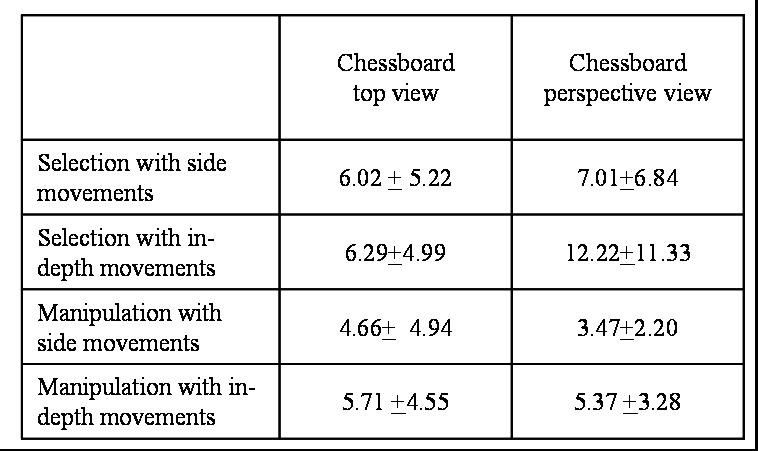
\includegraphics[width=.7\textwidth]{table.jpg}
%\end{table}


\section{References}

%Bibliographic references must be unambiguous and uniform.  We recommend giving
%the author names references in brackets, e.g. \cite{knuth:84},
%\cite{boulic:91}, and \cite{smith:99}.


\bibliographystyle{sbc}
\bibliography{sbc-template}

\end{document}
